\documentclass{article}
\usepackage{graphicx}
\usepackage{booktabs}
\usepackage{geometry}
\usepackage{float}
\usepackage{listings}
\usepackage{xcolor}
\usepackage{subcaption}
\usepackage{setspace}
\usepackage[slantfont,boldfont]{xeCJK}
\usepackage{fontspec}
\usepackage{longtable}
\usepackage{array}
\usepackage{hyperref}

\geometry{a4paper,scale=0.8}
\onehalfspacing
\hypersetup{colorlinks=true, linkcolor=black, urlcolor=blue}

\definecolor{dkgreen}{rgb}{0,0.6,0}
\definecolor{gray}{rgb}{0.5,0.5,0.5}
\definecolor{mauve}{rgb}{0.58,0,0.82}
\lstset{
frame=tb,
language=bash,
aboveskip=3mm,
belowskip=3mm,
showstringspaces=false,
columns=flexible,
basicstyle={\small\ttfamily},
numbers=left,
numberstyle=\tiny\color{gray},
keywordstyle=\color{blue},
commentstyle=\color{dkgreen},
stringstyle=\color{mauve},
breaklines=true,
breakatwhitespace=true,
tabsize=2
}

\title{实验五\hspace{2em}实验报告}
\author{人工智能2402\hspace{1em}陈子硕}
\date{May 2026}

\begin{document}

\maketitle

\section{实验环境说明}
本实验围绕“基于容器的云上训练和推理”展开，主要完成 Docker 基础操作、容器化 PyTorch 训练，以及基于 TorchServe 的推理服务部署。整体实验在 Linux 环境下完成，训练和推理均以 GPU 容器为主。

\begin{table}[H]
\centering
\caption{实验硬件环境}
\label{tab:hardware_env_exp5}
\begin{tabular}{p{0.28\linewidth} p{0.64\linewidth}}
\toprule
项目 & 配置 \\
\midrule
CPU & 通用多核处理器 \\
GPU & NVIDIA GPU \\
训练方式 & Docker 容器内运行 PyTorch 训练任务 \\
推理方式 & Docker 容器内运行 TorchServe 推理服务 \\
\bottomrule
\end{tabular}
\end{table}

\begin{table}[H]
\centering
\caption{实验软件环境}
\label{tab:software_env_exp5}
\begin{tabular}{p{0.28\linewidth} p{0.64\linewidth}}
\toprule
项目 & 配置 \\
\midrule
操作系统 & Linux 类系统 \\
容器引擎 & Docker Engine \\
训练框架 & PyTorch \\
推理服务 & TorchServe \\
CUDA 支持 & 通过 GPU 容器与 \texttt{--gpus all} 参数启用 \\
训练镜像 & \texttt{pytorch/pytorch:2.10.0-cuda12.6-cudnn9-devel} \\
推理镜像 & \texttt{pytorch/torchserve:latest-gpu} \\
\bottomrule
\end{tabular}
\end{table}

\section{实验目标与实验内容}
根据指导书要求，本实验的核心目标包括：
\begin{enumerate}
    \item 理解 Docker 的镜像、容器和隔离机制，熟悉基础容器操作流程；
    \item 掌握使用 Dockerfile 封装 PyTorch 训练环境的方法；
    \item 完成典型训练任务的容器化部署，并观察训练日志与模型收敛情况；
    \item 基于 TorchServe 完成模型归档、服务启动、健康检查与外部推理调用；
    \item 总结容器在环境一致性、部署便捷性和模型服务化中的工程价值。
\end{enumerate}

\section{实验过程与结果分析}
\subsection{Docker 基础操作}
实验开始阶段先验证 Docker 环境是否可用，主要执行镜像拉取、临时容器运行、交互式进入容器和容器状态查看等操作。基础命令如下：

\begin{lstlisting}[caption={Docker 基础操作命令},label={lst:docker_basic}]
docker pull alpine
docker images
docker run alpine ls -l
docker run -it alpine /bin/sh
docker ps
\end{lstlisting}

这一阶段的重点不是训练任务本身，而是熟悉 Docker daemon 拉取镜像、创建容器、执行命令并将结果返回给客户端的完整路径。通过交互式方式进入 Alpine 容器后，可以更直观地理解容器文件系统与宿主机环境之间的隔离关系。

\subsection{容器化 PyTorch 训练部署}
训练部分使用 PyTorch 官方镜像作为基础环境。按照指导书思路，可以通过 Dockerfile 固定镜像、设置工作目录、复制训练代码并设定容器启动命令。例如：

\begin{lstlisting}[caption={训练镜像 Dockerfile 示例},label={lst:dockerfile_train}]
FROM pytorch/pytorch:2.10.0-cuda12.6-cudnn9-devel
WORKDIR /workspace
COPY . /workspace
CMD ["python", "pytorch_mnist_example.py"]
\end{lstlisting}

镜像构建与训练启动命令如下：

\begin{lstlisting}[caption={训练镜像构建与运行},label={lst:docker_train_run}]
docker build -f Dockerfile -t train_dl .
docker run --rm -it --gpus all -v "$PWD":/workspace -w /workspace train_dl
\end{lstlisting}

从训练日志可见，MNIST 训练过程能够稳定收敛。第 3 个 Epoch 后，测试集平均损失约为 0.0396，准确率达到 9889/10000，即 98.89\%。这表明容器中的 PyTorch、CUDA 运行时与训练代码能够正确协同，训练任务具备较好的可复现性。

\begin{figure}[H]
    \centering
    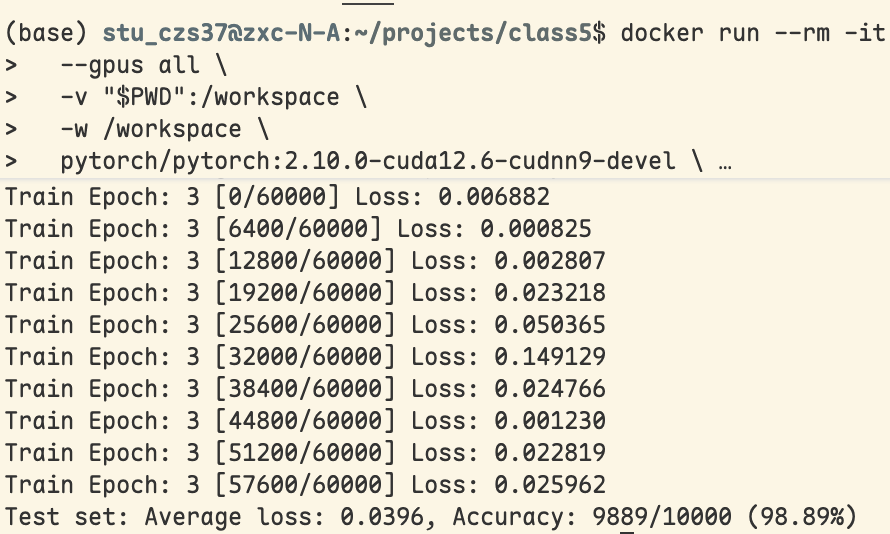
\includegraphics[width=0.95\linewidth]{截屏2026-05-16 15.18.45.png}
    \caption{使用 GPU 参数启动容器后的训练日志}
    \label{fig:train_gpu_log}
\end{figure}

\begin{figure}[H]
    \centering
    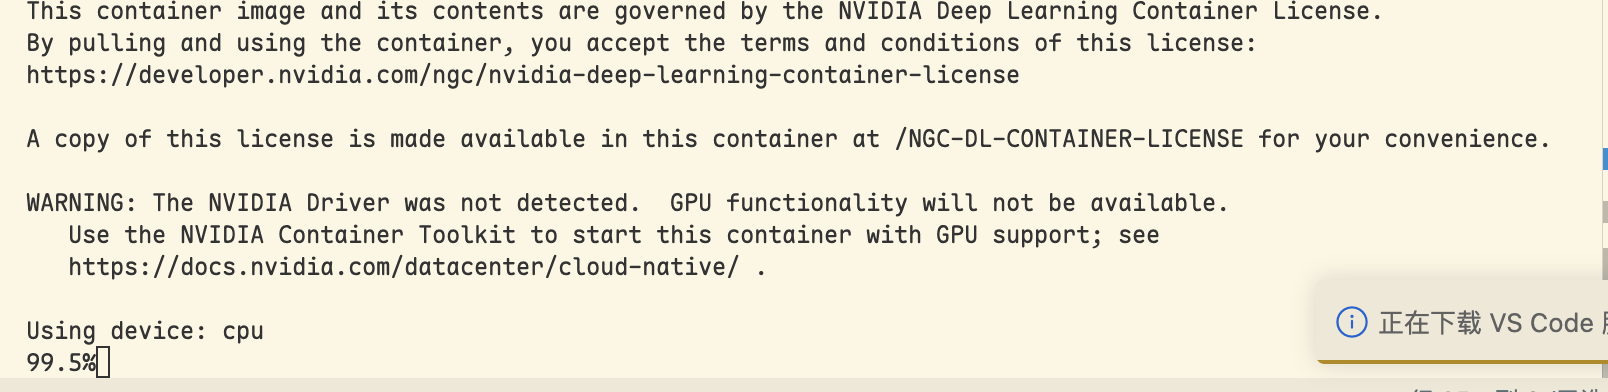
\includegraphics[width=0.95\linewidth]{截屏2026-05-16 15.15.40.png}
    \caption{未正确启用 GPU 时，容器内仅使用 CPU}
    \label{fig:cpu_warning}
\end{figure}

由图~\ref{fig:cpu_warning} 可以看出，若没有正确传递 GPU 资源，容器会提示 \texttt{NVIDIA Driver was not detected}，随后训练程序退回到 CPU 模式，这会显著增加训练时间开销。因此在深度学习任务中，\texttt{docker run} 阶段的 GPU 参数是容器化训练能否高效运行的关键条件。

\subsection{基于 TorchServe 的推理服务部署}
推理部分采用 TorchServe 官方 GPU 镜像，并对主机端口进行映射。为了在容器中访问 \texttt{model-archiver} 以及示例模型文件，我将宿主机上的 \texttt{serve} 项目目录直接挂载到容器内部：

\begin{lstlisting}[caption={TorchServe 容器启动命令},label={lst:torchserve_run}]
docker run --rm -it --gpus all \
  -p 8080:8080 -p 8081:8081 \
  -v $(pwd)/serve:/serve \
  --name torchserve_lab pytorch/torchserve:latest-gpu
\end{lstlisting}

随后在容器内下载 \texttt{densenet161} 权重，并使用 \texttt{torch-model-archiver} 生成 \texttt{densenet161.mar}：

\begin{lstlisting}[caption={模型归档过程},label={lst:model_archiver}]
cd /home/model-server/model-store
wget https://download.pytorch.org/models/densenet161-8d451a50.pth
cd /serve/model-archiver
pip install .
torch-model-archiver --model-name densenet161 --version 1.0 \
  --model-file /serve/examples/image_classifier/densenet_161/model.py \
  --serialized-file /home/model-server/model-store/densenet161-8d451a50.pth \
  --export-path /home/model-server/model-store \
  --extra-files /serve/examples/image_classifier/index_to_name.json \
  --handler image_classifier
\end{lstlisting}

模型归档完成后，停止旧的 TorchServe 实例，并重新启动推理服务：

\begin{lstlisting}[caption={TorchServe 服务启动与测试},label={lst:torchserve_start}]
torchserve --stop
torchserve --start --ncs --model-store model-store --models densenet161.mar --disable-token-auth
curl http://localhost:8080/ping
curl -X POST http://127.0.0.1:8080/predictions/densenet161 -T kitten.jpg
\end{lstlisting}

其中，\texttt{/ping} 接口用于健康检查；当返回 \texttt{\{"status":"Healthy"\}} 时，说明推理服务已经可用。之后通过 \texttt{predictions} 接口上传测试图片，可得到 JSON 形式的预测结果。该过程说明，经过模型归档和服务加载后，原本只能在脚本中调用的 PyTorch 模型已经转化为标准的 HTTP 推理服务。

\begin{figure}[H]
    \centering
    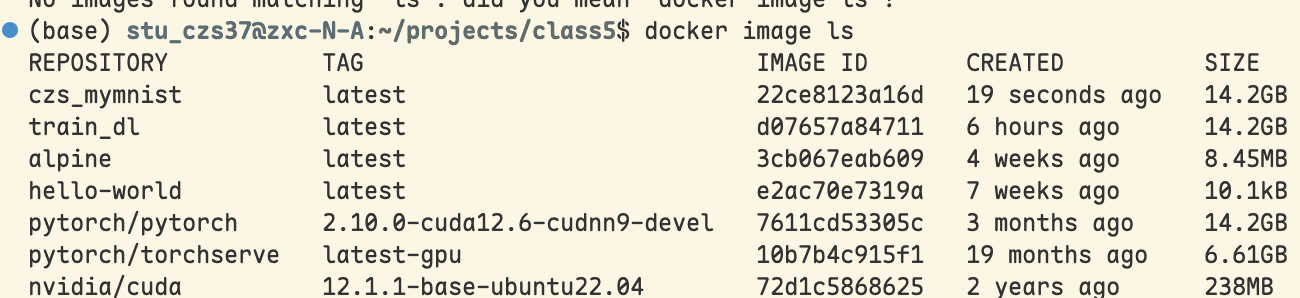
\includegraphics[width=0.95\linewidth]{截屏2026-05-16 15.12.07.png}
    \caption{实验过程中的 Docker 镜像与相关环境}
    \label{fig:docker_images}
\end{figure}

\section{实验中遇到的问题与解决方法}
\subsection{问题一：容器内找不到 \texttt{/serve/model-archiver}}
在执行 \texttt{cd /serve/model-archiver} 时，发现容器内并不存在该目录。排查后发现，TorchServe 官方运行镜像并不保证带有完整的源码目录，而模型归档命令中所需的 \texttt{model-archiver} 与示例文件路径依赖于 \texttt{serve} 项目源码。

解决方法是在宿主机先执行 \texttt{git clone https://github.com/pytorch/serve.git}，随后在启动容器时增加目录挂载参数：

\begin{lstlisting}[caption={挂载宿主机 serve 目录到容器},label={lst:mount_serve}]
docker run --rm -it --gpus all \
  -p 8080:8080 -p 8081:8081 \
  -v $(pwd)/serve:/serve \
  --name xxx pytorch/torchserve:latest-gpu
\end{lstlisting}

这样就能将主机文件夹映射到容器内，顺利访问 \texttt{/serve/model-archiver} 和 \texttt{/serve/examples}。

\subsection{问题二：\texttt{curl} 推理请求返回 400 错误}
在 TorchServe 启动后，用 \texttt{curl} 调用推理接口时出现了 400 错误。结合现象分析，这通常与 TorchServe 的 API 验证机制有关。停止原有服务后，在启动命令中加入 \texttt{--disable-token-auth} 参数即可禁用鉴权：

\begin{lstlisting}[caption={禁用 TorchServe API 验证},label={lst:disable_auth}]
torchserve --stop
torchserve --start --ncs --model-store model-store --models densenet161.mar --disable-token-auth
\end{lstlisting}

加入该参数后，再次执行 \texttt{curl} 推理请求即可正常返回预测结果。

\subsection{问题三：训练任务默认只使用 CPU}
实验 5 的训练任务在继承 PyTorch 镜像时，如果 \texttt{docker run} 没有明确指定 GPU，容器内程序将只在 CPU 上训练，造成明显更大的时间开销。这个问题从日志中也能直接观察到：容器提示未检测到 NVIDIA Driver，随后训练设备变成 \texttt{cpu}。

对应的解决方式是在训练容器启动时显式加入 GPU 参数：

\begin{lstlisting}[caption={训练任务显式启用 GPU},label={lst:gpu_enable}]
docker run --rm -it --gpus all \
  -v "$PWD":/workspace \
  -w /workspace \
  pytorch/pytorch:2.10.0-cuda12.6-cudnn9-devel
\end{lstlisting}

如果宿主机本身已正确安装 NVIDIA Driver 和 NVIDIA Container Toolkit，那么该命令即可让容器正常继承 GPU 计算能力。

\section{实验总结}
本次实验比较完整地走通了容器化深度学习任务的两条主线：一条是训练环境封装，另一条是模型服务化部署。训练部分说明 Dockerfile 能够把代码、依赖和启动命令打包为可重复使用的镜像；推理部分则说明 TorchServe 可以把训练好的 PyTorch 模型包装成标准 HTTP 服务，从而方便在云端或多用户环境中统一调用。

从工程化角度看，容器的最大优势在于环境一致性和迁移便利性。训练任务在不同机器上往往容易受到 Python 版本、CUDA 版本、依赖库差异的影响，而容器能够把这些环境因素固定下来，大幅降低“本机能跑、换机失效”的概率。与此同时，容器的端口映射、目录挂载和 GPU 资源传递机制，也为模型部署、实验复现和服务发布提供了清晰边界。

实验过程中遇到的三个问题也很有代表性：源码目录缺失说明容器镜像与源码仓库并不等价；推理接口 400 说明服务部署除了模型本身，还涉及接口访问策略；训练默认回退到 CPU 则说明硬件资源不会自动透传给容器。理解并解决这些问题后，我对容器化训练、云端部署和模型服务化之间的关系有了更直观的认识。

\end{document}
